\chapter{Dark energy and modified gravity in linear theory}\label{ch:extended-models}
\chapterstatus{written}{2026-11-17}

The Einstein--Boltzmann solver has a library of some twenty models beyond $\Lambda$CDM. Their backgrounds were
described in \cref{ch:background}; this chapter gives their perturbations. Every model uses the conventions of
\cref{ch:linear-perturbations} (Newtonian gauge, $x=\ln a$, $\Phi$ with the sign of Callin; below
$\Phi_P=-\Phi$ is the potential with the Planck sign) and is selected by \code{model = <name>} with its parameters in
the parameter file. The quasi-static limits of the theories, collected in \cls{QuasiStaticGravity}, are shared with the
growth factors, the one-loop hybrid bias and SimulationCode.

\begin{modulebox}{Cosmology/Perturbations (models)}
Species: \file{SpeciesPerturbation_ScalarField.h} (quintessence, EDE, axion), \file{_DarkEnergyFluid.h} (dark
scattering, IDE), \file{_CoupledQuintessence.h}, \file{_MassiveNeutrinos.h}, \file{_CDM.h},
\file{_MasslessNeutrinos.h}.\par
Field equations: \file{PerturbedFieldEquation_GeneralRelativity.h}, \file{_BransDicke.h}, \file{_MuSigma.h} (with
DGP and Hu--Sawicky), \file{_HorndeskiAlpha.h}, \file{_CubicGalileon.h}.\par
Quasi-static theories: \file{QuasiStaticGravity.h} and \file{QuasiStaticGravity_<name>.h} (MuSigma, HuSawicky,
DGP, BransDicke, Symmetron, Dilaton, MBeta, CubicGalileon, Horndeski).\par
Models and registry: \file{PerturbationModel_<name>.h}, \file{PerturbationModel_HorndeskiTable.h}, \file{Presets.h}.
Validation: \file{EinsteinBoltzmannSolver/DEVELOPING.md}, report Sec.~XI.
\end{modulebox}

\section{Quasi-static gravity}\label{sec:ext-quasistatic}

Far inside the horizon and neglecting time derivatives of the extra fields, a theory of gravity modifies the Poisson
equations for the comoving density $\rho\Delta$ of all species:
\begin{equation}
k^2\Psi=-4\pi Ga^2\,\mu(k,a)\,\rho\Delta,\qquad k^2(\Phi_P+\Psi)=-8\pi Ga^2\,\Sigma(k,a)\,\rho\Delta .
\label{eq:ext-musigma}
\end{equation}
$\mu=G_{\rm eff}/G$ is the force on non-relativistic matter (growth, $N$-body forces) and $\Sigma$ the lensing (Weyl)
potential; GR is $\mu=\Sigma=1$. \cls{QuasiStaticGravity} gives, on any \cls{Background},
\begin{itemize}
\item \code{mu_sigma(x, k)}: $\mu$, $\Sigma$ and $\dd(2\Sigma-\mu)/\dd x$ at fixed $k$ (needed by the solver);
\item \code{second_order_source(x, k)}: the $D_1^2$ source of the 2LPT growth equation relative to GR,
      $D_2''+(2+\frac{\dd\ln H}{\dd x})D_2'=\frac32\Om_m(a)\mu\,(D_2-s_2D_1^2)$ ($s_2=1$ in GR and in theories without a
      nonlinear term; smaller with Vainshtein screening);
\item \code{screening()}: the type (Newtonian potential for chameleon-like theories, density for Vainshtein, gradient
      for k-mouflage) and the surviving fraction of the fifth force as a function of that quantity, used by the
      approximate screening methods of SimulationCode (\cref{ch:mg-simulations}).
\end{itemize}
$k$ is in units of $H_0/c$ (\code{koverH0}). The theories are summarised in \cref{tab:ext-qs}.

\begin{table}[htbp]
\centering\small
\caption{Quasi-static theories. $\beta$ and $m$ are the coupling and mass of a scalar fifth force; screening factors
are $\min(1,\epsilon\,\Phi_{\rm crit}/|\Phi_N|)$ for potential screening, with an efficiency $\epsilon$.}
\label{tab:ext-qs}
\begin{tabularx}{\textwidth}{@{}lXX@{}}
\toprule
Theory & $\mu(k,a)$, $\Sigma$ & Screening \\
\midrule
$\mu$--$\Sigma$ (Planck/DES) & $\mu=1+\mu_0\frac{\Om_{\rm DE}(a)}{\Om_{\rm DE,0}}$, $\Sigma=1+\Sigma_0\frac{\Om_{\rm DE}(a)}{\Om_{\rm DE,0}}$ & --- \\
Hu--Sawicky $f(R)$ & $\frac{1+\frac13\frac{k^2}{k^2+a^2m^2}}{1+f_R}$, $\Sigma=\frac{1}{1+f_R}$ & potential, $\Phi_{\rm crit}=\frac32|f_R(a)|$ \\
DGP & $1+\frac{1}{3\beta}$, $\beta=1-2\epsilon\frac{Hr_c}{c}\left(1+\frac{\dd\ln H}{3\dd\ln a}\right)$, $\Sigma=1$ & Vainshtein (density) \\
Cubic Galileon & $\mu=\Sigma=1+\frac{\Om_\phi(a)}{1-2\frac{\dd\ln H}{\dd\ln a}-\Om_\phi(a)}$ & Vainshtein (density) \\
Brans--Dicke & from the sub-horizon field equations, $G_{\rm eff}=G\phi_*/\phi$ & --- \\
Symmetron & $1+\frac{2\beta^2(a)k^2}{k^2+a^2m^2(a)}$ after $a_{\rm ssb}$, $\Sigma=1$ & potential \\
Dilaton & as symmetron with $m=m_0a^{-r}$, $\beta=\beta_0e^{s(a^p-1)/p}$ & potential, $\Phi_{\rm crit}=1/(2A_2)$ \\
$(m,\beta)$ & as symmetron with $\beta=\beta_0a^{n_\beta}$, $m=m_0a^{n_m}$ & potential \\
Horndeski (table) & from the $\alpha$'s of the reduced theory \cite{Kimura2012} & Vainshtein \\
\bottomrule
\end{tabularx}
\end{table}

\paragraph*{Hu--Sawicky $f(R)$} \cite{HuSawicki2007}. In the high-curvature regime $f_R=-|f_{R0}|(R_0/R)^{n+1}$ and
$f_{RR}=-(n+1)f_R/R$, with the background Ricci scalar $Rc^2/(3H_0^2)=2E^2(2+\dd\ln E/\dd x)-2\Om_ke^{-2x}$ (the
$\order{f_{R0}}$ corrections to the expansion are neglected, as in MGCAMB). The scalaron mass is
$m^2c^2/H_0^2=(1+f_R)\,Rc^2/[3H_0^2(n+1)|f_R|]$, and $Q=(k/a)^2f_{RR}/(1+f_R)=(k/a)^2/(3m^2)$ gives the familiar
$\mu=(1+4Q)/[(1+3Q)(1+f_R)]$: gravity is enhanced by $4/3$ below the Compton wavelength $1/m$.

\paragraph*{DGP} \cite{KoyamaMaartens2006}. The brane-bending mode strengthens gravity on the normal branch
($\epsilon=-1$) and weakens it on the self-accelerating branch; it does not change the lensing potential. $H(a)$ is
that of the background, whichever it is. The nonlinear term of the field equation gives
$s_2=1-2(r_cH_0/c)^2\rho_m(a)/(9\beta^3\mu)$. For a spherical top-hat the fifth force is reduced by
$2(\sqrt{1+e}-1)/e$ with $e=8(r_cH_0/c)^2\rho_m\delta/(9\beta^2)$; the screening approximation used by default replaces
$\rho_m(a)$ by $\Om_m$ and $\delta$ by $1+\delta$, which reproduces the exact multigrid $P(k)$ better (0.5\% against
1.2\% rms at $z=0$).

\paragraph*{Cubic Galileon.} On the tracker the quasi-static scalar equation is that of DGP's brane-bending mode
with a time-dependent crossover scale, $\beta=(1-2\varepsilon-\Om_\phi(a))/(3\Om_\phi(a))$ and
$(r_cH_0/c)^2=E^2/(2\Om_\phi(a)\Om_{\phi0})$, $\varepsilon=\dd\ln H/\dd\ln a$ \cite{Barreira2013}; the Galileon enters
$\Phi$ and $\Psi$ alike, so $\Sigma=\mu$ ($\mu=1.77$ today for $\Om_{\phi0}=0.68$). In voids ($e<-1$) there is no real
solution and $e=-1$ is used, as in the multigrid solver.

\paragraph*{Symmetron, dilaton and $(m,\beta)$} \cite{Brax2012}. These chameleon-like theories have a scalar of mass
$m(a)$ coupled to matter with strength $\beta(a)$ and $\mu=1+2\beta^2k^2/(k^2+a^2m^2)$. The symmetron
\cite{Brax2012}, generalised to the powers $(N,M)$ (even, $M>N\ge2$; $(2,4)$ is the original) with
$V\propto-\frac1N(\phi/\phi_*)^N+\frac1M(\phi/\phi_*)^M$, has no fifth force before symmetry breaking at $a_{\rm ssb}$ and
\begin{equation}
\chi=\frac{\phi}{\phi_*}=\left[1-(a_{\rm ssb}/a)^3\right]^{\frac{1}{M-N}},\quad \beta(a)=\beta\chi^{N-1},\quad
m^2=\frac{\chi^{N-2}\left[1-(a_{\rm ssb}/a)^3\right]}{(H_0L/c)^2}\frac{H_0^2}{c^2},
\end{equation}
with the vacuum range $L$ (\param{sym_assb}, \param{sym_beta}, \param{sym_L_mpch}, \param{sym_N}, \param{sym_M}). The
environment-dependent dilaton has $A(\phi)=1+A_2\phi^2/(2\Mpl^2)$, $m=m_0a^{-r}$ ($r\le3/2$) and
$\beta(a)=\beta_0\exp[s(a^p-1)/p]$ with $p=2r-3$, $s=9\Om_mA_2\xi^2$, $\xi=H_0/m_0$ (\param{dil_A2},
\param{dil_beta0}, \param{dil_r}, \param{dil_xi}). The $(m,\beta)$ parameterisation uses power laws
(\param{mb_beta0}, \param{mb_n_beta}, \param{mb_m0}, \param{mb_n_m}); its screening threshold
$\Phi_{\rm crit}=\phi(a)/(2\beta\Mpl)$ needs the background field $\phi/\Mpl=9\Om_m\int_0^a\beta/(a'^3(m/H_0)^2)\,
\dd\ln a'$.

\paragraph*{In the Einstein--Boltzmann solver} the quasi-static theories (\code{musigma}, \code{dgp}, \code{fr},
\code{symmetron}, \code{dilaton}, \code{mbeta}) use the $\mu$--$\Sigma$ field equations. On super-horizon scales
$\rho\Delta\sim(k/\Hp)^2\delta\rho$, so computing the potentials directly from \cref{eq:ext-musigma} would lose all
precision there. Instead the GR potential of the comoving density, $\Phi_{\rm GR}=\frac32H_0^2a^2\rho\Delta/
(\rho_{c0}c^2k^2)$, is evolved with the equation that follows from energy--momentum conservation of all species
(with $A=3/(2c^2k^2)$ and densities times $H_0^2a^2$),
\begin{multline}
\Phi_{\rm GR}'\left[1+3A(\rho+p)(2\Sigma-\mu)\right]=-\Phi_{\rm GR}+A\Big[-\frac{ck}{\Hp}\,{\rm flux}
+3\left(\frac{\Hp'}{\Hp}-1\right)\frac{\rm flux}{ck/\Hp}-2\,{\rm shear}\\+3(\rho+p)\Psi-3(\rho+p)(2\Sigma-\mu)'\Phi_{\rm GR}\Big],
\end{multline}
and $\Psi=-\mu\Phi_{\rm GR}-S$, $\Phi=(2\Sigma-\mu)\Phi_{\rm GR}$ with $S$ the anisotropic stress term. The GR energy
constraint minus its momentum-constraint form is added, so $\mu=\Sigma=1$ is exactly the GR code. These models require
a flat universe and $2\Sigma-\mu\ge0$.

\section{Scalar fields: quintessence, early dark energy and axions}\label{sec:ext-scalar}

The field perturbation $\delta\phi$ obeys the Klein--Gordon equation in Newtonian gauge. With
$w\equiv\delta\phi_x-\phi_x\Psi$, which removes $\Psi'$,
\begin{align}
\delta\phi_x&=w+\phi_x\Psi,\\
w_x&=-\left(2+\frac{\Hp'}{\Hp}\right)w-\left(\frac{ck}{\Hp}\right)^2\delta\phi-\frac{3v_{\phi\phi}}{E^2}\delta\phi
-3\phi_x\Phi'-\frac{3v_\phi}{E^2}\Psi,
\end{align}
with the moments (times $H_0^2a^2/\rho_{c0}$) $\delta\rho=\Hp^2\phi_xw/3+H_0^2a^2v_\phi\delta\phi$,
$\delta p=\Hp^2\phi_xw/3-H_0^2a^2v_\phi\delta\phi$, flux $=(ck/\Hp)\Hp^2\phi_x\delta\phi/3$ and no anisotropic stress.
The frozen field starts with $\delta\phi=w=0$.

\paragraph*{The oscillating field as a fluid.} When the background replaces a fast-oscillating field by a fluid
(\cref{sec:bg-scalar-fields}), the perturbations switch at the same $x$ to the effective fluid of an oscillating
field \cite{Poulin2018}, with $w=c_a^2=w_{\rm osc}$ and the rest-frame sound speed
\begin{equation}
c_s^2(k,x)=\frac{2(n-1)W+(ck/\Hp)^2}{2(n+1)W+(ck/\Hp)^2},\qquad W=(\varpi/H)^2,
\end{equation}
for $V\propto|\phi-\phi_{\min}|^{2n}$ ($n=1$: the ultralight axion, $c_s^2=k^2/(k^2+4m^2a^2)$), where $\varpi$ is the
angular frequency of the oscillation, computed from the period of the actual potential at the switch and scaled as
$\rho^{(n-1)/2n}$ afterwards. The fluid obeys the dark-energy fluid equations below. At the switch $(\delta\phi,w)$ is
split into a shift along the trajectory, which carries the momentum, and a change of amplitude; the density is set
from the comoving density perturbation, which is continuous and does not oscillate, so the Einstein constraints hold
exactly through the switch (the neglected terms are $\order{H/m}<10^{-2}$ of the field's perturbation). For the axion
with \param{ax_switch_mH} $\le4$ the switch keeps axionCAMB's synchronous-gauge $\delta$ and $(1+w)v$ continuous.

\section{Dark-energy fluids and dark-sector interactions}\label{sec:ext-fluids}

A dark-energy fluid of constant $w$ and rest-frame sound speed $\hat c_s^2$ (variables $\delta_{\rm DE}$ and
$u=\theta/(ck)$) obeys
\begin{align}
\delta_{\rm DE}'&=-(1+w)\left(\frac{ck}{\Hp}u+3\Phi'\right)-3(\hat c_s^2-w)\left[\delta_{\rm DE}+\frac{3(1+w)u}{ck/\Hp}\right],\\
u'&=-(1-3\hat c_s^2)u+\frac{ck}{\Hp}\left[\frac{\hat c_s^2\delta_{\rm DE}}{1+w}+\Psi\right],
\end{align}
with $\delta p_{\rm DE}=\rho_{\rm DE}[\hat c_s^2\delta_{\rm DE}+3(1+w)(\hat c_s^2-w)u/(ck/\Hp)]$. It is evolved in one block
with the CDM it interacts with.

\paragraph*{Dark scattering} \cite{Simpson2010,BaldiSimpson2015} exchanges only momentum:
\begin{gather}
v_c'=-v_c-\frac{ck}{\Hp}\Psi+\frac{\Gamma_c}{\Hp}(v_{\rm DE}-v_c),\qquad u'=\ldots-\frac{\Gamma_{\rm DE}}{\Hp}(u-u_c),\\
\Gamma_{\rm DE}=ac\,\xi\rho_c,\qquad \Gamma_c=(1+w)\frac{\rho_{\rm DE}}{\rho_c}\Gamma_{\rm DE}.
\end{gather}
While $\Gamma_{\rm DE}/\Hp>200$ the dark-energy velocity is locked to that of the dark matter (its momentum is negligible
then). The covariant dark Thomson-like scattering has $\Gamma_c=\alpha H_0a^4/\Om_{c0}$. Parameters: \param{ds_w},
\param{ds_xi}, \param{ds_cs2}; $\xi=0$ is $w$CDM with dark-energy perturbations.

\paragraph*{Interacting dark energy} \cite{Valiviita2008} transfers energy along the dark-matter four-velocity, with
the perturbed rate from the local expansion of the dark matter, $\delta Q/Q=\delta_{\rm DE}-\Psi+E$,
$E=-\frac13\frac{ck}{\Hp}v_c+\Phi'$, and the doom factor $d=\xi/[3(1+w)]$:
\begin{align}
\delta_c'&=\frac{ck}{\Hp}v_c-3\Phi'+\xi\frac{\rho_{\rm DE}}{\rho_c}(\delta_{\rm DE}-\delta_c+E),\qquad v_c'=-v_c-\frac{ck}{\Hp}\Psi,\\
\delta_{\rm DE}'&=-(1+w)\left(\frac{ck}{\Hp}u+3\Phi'\right)-3(\hat c_s^2-w)\left[\delta_{\rm DE}+\frac{3(1+w)(1+d)u}{ck/\Hp}\right]-\xi E,\\
u'&=\left[3\hat c_s^2-1+3d(\hat c_s^2-w)\right]u+\frac{ck}{\Hp}\left[\frac{\hat c_s^2\delta_{\rm DE}}{1+w}+\Psi\right]+\xi u+3dv_c .
\end{align}
The early-time instability \cite{Valiviita2008} is avoided for $d<0$; the code rejects $d>0$ (\param{ide_stability_check})
and backgrounds with $\rho_c<0$ before today.

\paragraph*{Coupled quintessence} \cite{Wetterich1995,Amendola2000} evolves the CDM and the field in one block:
\begin{align}
\delta_c'&=\frac{ck}{\Hp}v_c-3\Phi'-\beta\,\delta\phi_x,\qquad
v_c'=-(1-\beta\phi_x)v_c-\frac{ck}{\Hp}\Psi+\beta\frac{ck}{\Hp}\delta\phi,\\
w'&=\ldots-\frac{3(v_\phi-\beta\rho_c)}{E^2}\Psi+\frac{3\beta\rho_c}{E^2}\delta_c,
\end{align}
i.e.\ a fifth force that makes the effective gravitational constant of the dark matter $G(1+2\beta^2)$ on small
scales, and a drag $\propto\beta\phi_xv_c$. The Fading Dark Sector \cite{ObiedVafaWu2026} (\code{fading_dark_sector},
\cref{sec:bg-coupledquintessence}) uses these perturbations with $\lambda=c$, $\beta=c'$; its quasi-static limit
$G_{\rm eff,\chi\chi}=G[1+2c'^2k^2/(k^2+a^2m_{\rm eff}^2)]$ is the $k\gg am_{\rm eff}$ limit $1+2\beta^2$ here, since
$m_{\rm eff}\sim H$.

\section{Scalar--tensor theories with full perturbations}\label{sec:ext-scalartensor}

\paragraph*{Brans--Dicke.} The perturbations ($\Phi$, $\delta\phi$, $\delta\phi'$) are evolved in full (derived
symbolically), with the background of \cref{sec:bg-bransdicke}; \code{quasi_static()} gives their sub-horizon limit.

\paragraph*{Cubic Galileon.} The braided scalar perturbations of the tracker are evolved in full, derived covariantly
and checked with the identity $\nabla^\mu T_{\mu\nu}=(\nabla\cdot J)\phi_\nu$.

\paragraph*{Horndeski in the $\alpha$ basis.} Following Bellini and Sawicki \cite{Bellini2014} and hi\_class
\cite{Zumalacarregui2017}, the linear theory is described by the kineticity $\alpha_K$, the braiding $\alpha_B$, the
running of the Planck mass $\alpha_M=\dd\ln M_*^2/\dd\ln a$ and the background; $\alpha_T=0$ (GW170817). The
Newtonian-gauge equations were derived for $L=F(\phi)R/2+G_2(\phi,X)-G_3(\phi,X)\Box\phi$, which realises any
$(\alpha_K,\alpha_B,\alpha_M)$, the $G_i$ eliminated with the definitions of the $\alpha$'s and the background
equations, and the system reduced to first order in $v=-\delta\phi/\phi'$ and $u=v'+\Psi$. The no-ghost and gradient
stability conditions
\begin{equation}
D=\alpha_K+\tfrac32\alpha_B^2>0,\qquad
Dc_s^2=(2-\alpha_B)\left[\frac{\alpha_B}{2}+\alpha_M-\frac{\dot H}{H^2}\right]-\frac{\rho_m+p_m}{H^2M_*^2}+\frac{\dot\alpha_B}{H}>0
\end{equation}
and a stiffness bound $c_s^2\le10^5$ are checked (\param{hd_stability_check}). The parameterisations are those of
hi\_class, $\alpha_X=c_X f(a)$ with $f=\Om_{\rm DE}(a)$, $a$ or 1 (\param{hd_parametrization}, \param{hd_cK},
\param{hd_cB}, \param{hd_cM}, \param{hd_M2_ini}), on a $\Lambda$CDM or $w_0w_a$ expansion (\param{hd_w0},
\param{hd_wa}); $\alpha_K=\alpha_B=0$ with $\alpha_M\neq0$ is rejected. \code{horndeski_table} uses the $\alpha$'s of a
reduced Horndeski theory given by its Lagrangian (\cref{ch:background}); the cubic Galileon built this way reproduces
\code{cubic_galileon} to $2\times10^{-5}$ in $P(k)$.

\section{Model summary and validation}

\begin{table}[htbp]
\centering\small
\caption{The models beyond $\Lambda$CDM, the parameters used for \cref{fig:ext-models}, their perturbations and
validation, and $\sigma_8$ and $P(k=0.1\hMpc)$ relative to $\Lambda$CDM with the same primordial spectrum,
$\Om_b$, $\Om_c$ and $h$ (from the solver report).}
\label{tab:ext-models}
\begin{tabularx}{\textwidth}{@{}llXlcc@{}}
\toprule
Model & Parameters & Perturbations & Main validation & $\frac{\sigma_8}{\sigma_8^{\Lambda}}$ & $\frac{P}{P^{\Lambda}}$ \\
\midrule
quintessence & $\lambda=1$ & full field & constraints, background & 0.978 & 0.956 \\
coupled quint. & $\lambda=0.5$, $\beta=0.05$ & field + CDM & constraints, growth & 1.037 & 1.071 \\
dark scattering & $w=-0.9$, $\xi=10$\,b/GeV & fluid + CDM & CLASS ($\xi=0$), drag & 0.962 & 0.925 \\
EDE & $f_{\rm EDE}=0.12$, $z_c=3630$ & full field & CLASS\_EDE & 0.945 & 0.899 \\
IDE & $\xi=-0.1$, $w=-0.95$ & fluid + CDM & constraints, $w$CDM limit & 1.124 & 1.254 \\
$\mu$--$\Sigma$ & $\mu_0=0.3$, $\Sigma_0=0.1$ & $\mu$--$\Sigma$ & growth equation & 1.038 & 1.077 \\
nDGP & $H_0r_c/c=1$, $\Lambda$CDM bg. & quasi-static & growth equation & 1.070 & 1.145 \\
sDGP & $\Om_\Lambda=0$ & quasi-static & growth equation & 0.809 & 0.654 \\
Brans--Dicke & $\omega=100$ & full field & constraints, $G_{\rm eff}$ & 1.043 & 1.093 \\
$f(R)$ & $|f_{R0}|=10^{-5}$, $n=1$ & quasi-static & scale-dep.\ growth & 1.073 & 1.066 \\
cubic Galileon & --- & full (braiding) & constraints, $G_{\rm eff}$ & 1.097 & 1.203 \\
Horndeski & $c_K=1$, $c_B=0.6$, $c_M=0.3$ & full ($\alpha$ basis) & hi\_class, 3 theories & 1.020 & 1.040 \\
\bottomrule
\end{tabularx}
\end{table}

\begin{figure}[htbp]
\centering
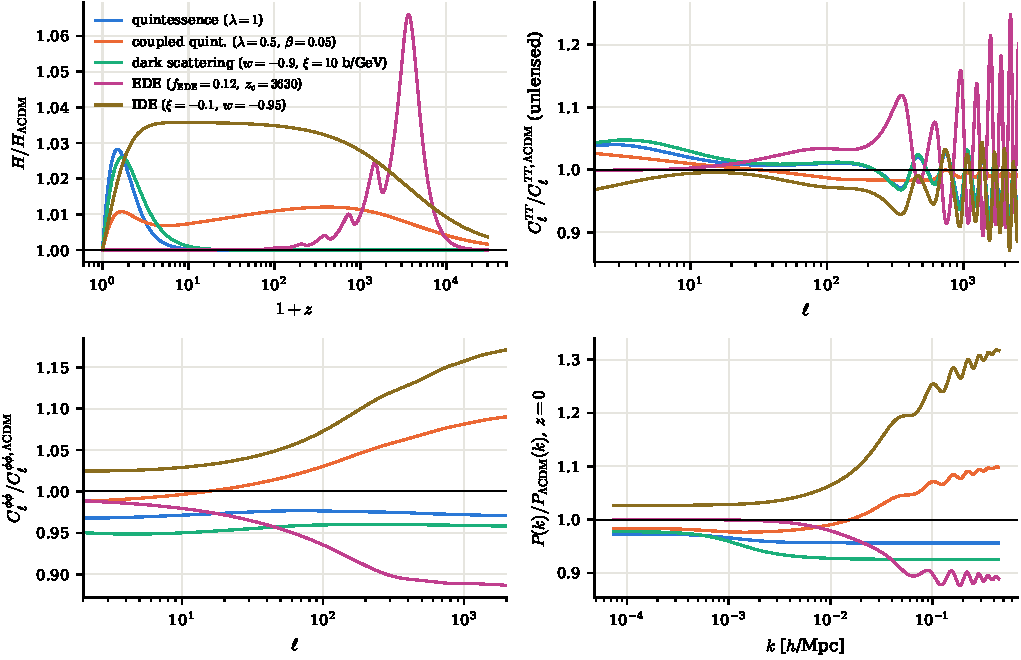
\includegraphics[width=\textwidth]{models_de}\\[2mm]
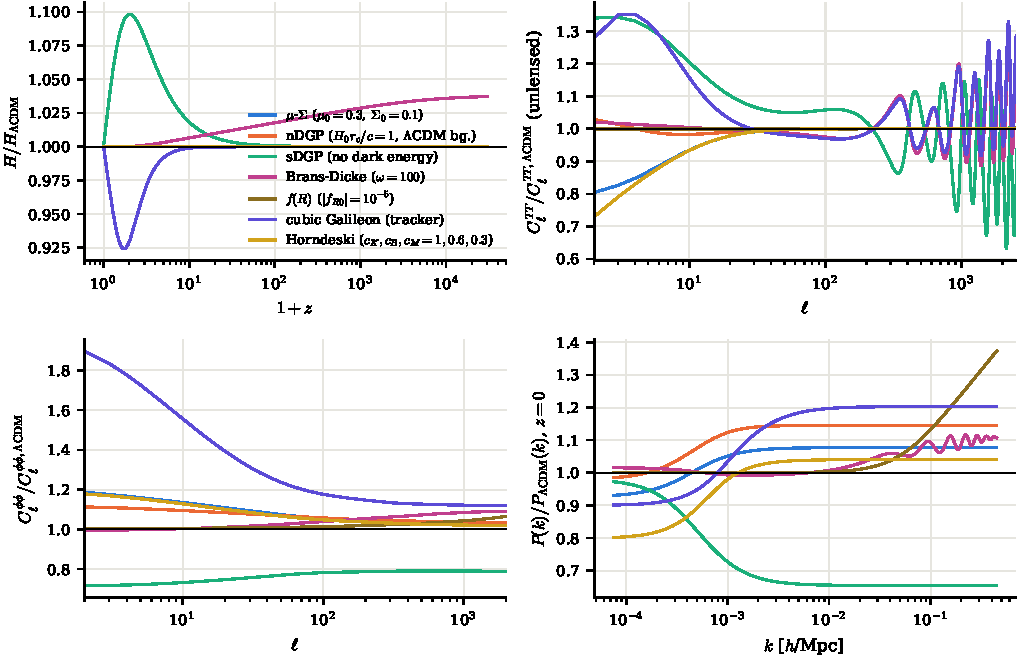
\includegraphics[width=\textwidth]{models_mg}
\caption{Dark-energy and dark-sector models (\emph{top}) and modified-gravity models (\emph{bottom}) relative to
$\Lambda$CDM: expansion rate, unlensed TT, lensing potential and $P(k)$ today, for the parameters of
\cref{tab:ext-models}. From the solver report.}
\label{fig:ext-models}
\end{figure}

\begin{validation}
Every model is tested in its GR/$\Lambda$CDM limit and, where possible, with the Einstein constraints that are not
integrated (momentum constraint to $10^{-8}$--$10^{-6}$; in interacting models the constraint holds only if the
exchange cancels between the species), with independent solutions of the quasi-static growth equation
($10^{-4}$--$7\times10^{-5}$), and against external codes: CLASS's fluid dark energy ($w$CDM, $P(k)$ to
$5\times10^{-5}$), CLASS\_EDE (ratios to $\Lambda$CDM to $3\times10^{-5}$ in $P(k)$ at $k\le0.05\hMpc$ and $10^{-3}$ in
TT), hi\_class (ratios to $10^{-4}$ in $P(k)$, $8\times10^{-4}$ in TT) and axionCAMB (axion isocurvature transfer to
$3\times10^{-3}$). The Horndeski $\alpha$ implementation reproduces the dedicated cubic Galileon ($5\times10^{-9}$),
quintessence ($2\times10^{-11}$) and Brans--Dicke ($9\times10^{-9}$) implementations. Details:
\file{EinsteinBoltzmannSolver/DEVELOPING.md}.
\end{validation}

\begin{paramfile}[Running a model]
./cmb params/fr.ini                                    # Hu-Sawicky f(R) (pert_k_max = 1, los_k_max = 0.3)
./cmb model=horndeski hd_cK=1 hd_cB=0.6 hd_cM=0.3 lensing=true
./cmb model=ede ede_fEDE=0.12 ede_log10zc=3.56 ede_theta_i=2.83
\end{paramfile}
